\documentclass[12pt, letterpaper]{report}
\usepackage{graphicx}
\usepackage{hyperref}
\usepackage{amssymb}
\usepackage{amsmath}
\usepackage{float}
\usepackage{mathtools}
\usepackage{enumitem}
\usepackage{matlab-prettifier}
\usepackage{listings}
\usepackage[margin=1in]{geometry}
\usepackage[figurename=Figura]{caption}
\title{Actividad: Simulador de Coulomb}
\author{Juan Pablo Guerrero Escudero, A01706810}
\date{13 abril, 2024}
\begin{document}
\maketitle
\subsection*{Código fuente}
\begin{verbatim}
    % Script Coulomb
%Limpia todas las figuras, variables y terminal de Matlab. 
clc, clear, close all 

%Se le pide al usuario el número de cargas
num_charges = input('Cuántas cargas tiene el sistema? '); 
%Se crea una matriz de ceros para guardar las coordenadas en x, y, z, y la
%magnitud de cada carga. 
matrix_charges  = zeros(num_charges, 4); 
matrix_forces = zeros(num_charges, 4); 
%Se crea la constante K. 
k_constant = 8.98e9; 

%For loop desde 1 al número de cargas
for i = 1:num_charges
    %El usuario ingresa la magnitud y posición en x, y, z de cada carga
    fprintf('Ingresa los datos siguientes de la carga %d: \n', i)
    magnitude = input('Ingresa la magnitud de la carga en Coulombs. Para notación científica, por ejemplo (3.5e-6) ');     
    position_xyz = input('Ingresa la posición de la carga en formato [x y z]: '); 
    %Los inputs son ingresados a matrix_charges 
    matrix_charges(i, :) = [position_xyz, magnitude]; 
end
% Se le pregunta al usuario la carga de prueba sobre la que los cálculos se
% harán
test_charge = input('Sobre qué carga quieres calcular la fuerza neta? ');
%Por medio de un for loop, se calculan los vectores de separación y sus
%magnitudes. 
for i = 1:num_charges
    %Si el índice i y el número en test_charge son diferentes
    if ne(i, test_charge)
        separation_vector = matrix_charges(test_charge, 1:3) - matrix_charges(i, 1:3);
        %Igual, las coordenadas resultantes se añaden a matrix_forces
        matrix_forces(i, 1:3) = separation_vector; 
        %Se calcula la longitud de cada vector separación 
        % usando la función norm(), y se añade a la última columna de
        matrix_forces(i, 4) = norm(separation_vector); 
    end
end

%Se crea la variable resulting_force para guardar coordenadas de fuerza
%neta. 
resulting_force = [0, 0, 0]; 
%For loop de 1 al número de cargas. 
for i= 1: num_charges
    %Si el índice de i y la carga de prueba son diferentes
    if ne(i, test_charge)
        %Calcula (Q_i/R_i) * vector de separación R_
        force_component = (k_constant * matrix_charges(i, 4) * matrix_charges(test_charge, 4)) / (matrix_forces(i, 4)^3) * matrix_forces(i, 1:3); 
        %añade el resultado a la fuerza resultante
        resulting_force = resulting_force + force_component;
    end
end
    

fprintf('La fuerza neta sobre la carga %d es: %.2f N en la dirección [%.2f, %.2f, %.2f]\n', test_charge, norm(resulting_force), resulting_force(1), resulting_force(2), resulting_force(3))

\end{verbatim}
\subsection*{Descripción del programa}
El programa consiste en un simulador de la ley de Coulomb por medio de Matlab. Lo que hace es calcular 
la fuerza eléctrica neta ejercida sobre una carga puntual por todas las demás cargas del sistema. Entonces, consiste de varias partes: 
La primera parte le solicita al usuario, por medio de inputs el número de cargas del sistema, y crea dos matrices de ceros, con tamaño no. cargas x 4. En la primera 
matriz, llamada $matrix charges$ se guardan las coordenadas en x, y, y z, y la magnitud de cada carga, las cuales el usuario ingresa 
por medio de un for loop que pide cada una. La segunda matriz, llamada $matrix forces$ guarda las coordenadas de cada vector separación, así como su 
magnitud. \\ 

Una vez que el usuario ingresa todas las coordenadas de las cargas, la segunda parte del programa consiste en un for loop, que 
en primera instancia verifica que el índice de cada iteración sea diferente al de la carga de prueba seleccionada por el usuario. A partir de ahí, verifica 
el signo de cada par de cargas, y en caso de ser positivo o negativo, calcula el vector separación de diferente manera. Además, por medio de la función $norm()$ de Matlab, 
calcula la magnitud de cada vector separación. Una vez teniendo esos dos datos, en cada iteración guarda las coordenadas y magnitud en la matrix $matrix forces$. \\

En la tercera y última parte del programa, por medio de un for loop que corre de 1 hasta el número de cargas, verifica si el índice de cada iteración y el índice de la carga 
de prueba son diferentes. En ése caso, usa la siguiente fórmula para calcular la fuerza resultante de cada par de partículas: 
\begin{align}
F_{neta} = Kq_1((\frac{Q_2}{{R^3}_1})(\vec{R_1}) + (\frac{Q_3}{{R^3}_2})(\vec{R_2}) + (\frac{Q_3}{{R^3}_3})(\vec{R_3}) ... (\frac{Q_n}{{R^3}_n})(\vec{R_n}))
\end{align}
Ésta fórmula corresponde a la Ley de Coulomb, factorizando los términos comúnes en la suma vectorial de fuerzas eléctricas, que son $kq_1$, siendo $q_1$ la carga de prueba seleccionada. 
Por medio de un for loop, calcula cada fuerza neta entre par de partículas, y lo añade a una variable $resulting force$. Ésta, al final se le muestra al usuario con su dirección y magnitud. 

\subsection*{Ejemplos de ejecución}
\begin{enumerate}
\item Caso de prueba con $Q_1 = 3x10^{-6} C$, $Q_2 = 1.2x10^{-5} C$, con posición $Q_1 = [-1, 0, 0]$ y $Q_2 = [1, 0, 0]$. Carga de prueba siendo $Q_1$: 
\begin{figure}[H]
    \centering
    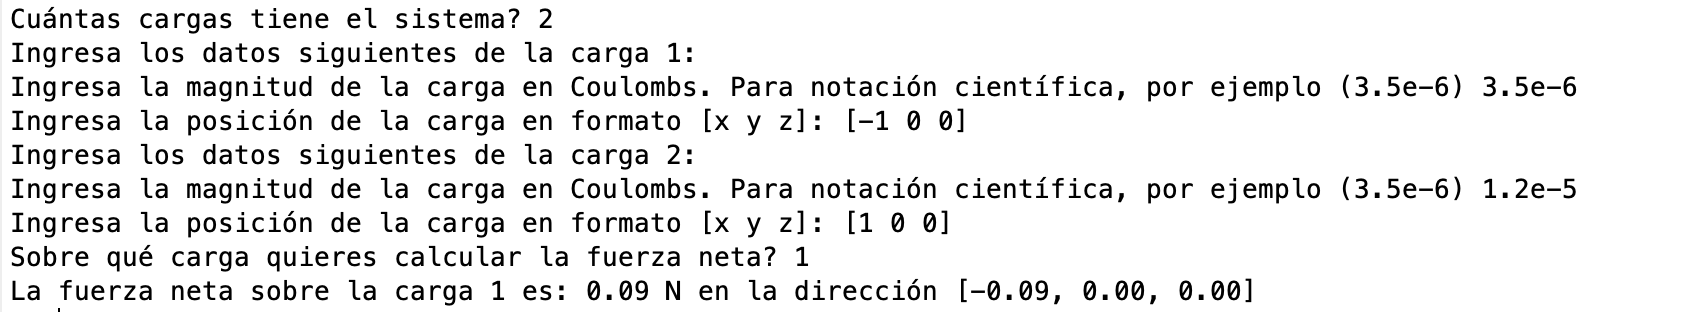
\includegraphics[height = 3 cm]{2024-04-11_Prueba1SimuladorCoulomb_1.png}
    \caption{Dos cargas separadas por dos metros de longitud}
    \label{fig:fig_1}
\end{figure}
En la figura \ref{fig:fig_1} se le pide al usuario ambas cargas de prueba, las cuáles son ingresadas en notación científica. A continuación, se le muestran los 
resultados de la carga neta ejercida sobre una carga particular. En éste caso, la fuerza neta es de $0.089N$, lo cuál hace sentido, ya que la magnitud es de tamaño correcto, 
y es positiva, lo que debería de ser si las dos partículas tienen carga positiva, ya que la fuerza es repulsiva entonces. Además, las coordenadas de la fuerza neta son correctas, 
ya que al solo tener posición en el eje $X$ las partículas, la fuerza debe estar en el eje $X$ también, lo cuál se cumple. \\

\item Caso de prueba con $Q_1 = 2x10^{-6}$ C, $Q_2 =-3x10^{-6} C, Q_3 = 1.5x10^{-6} C, Q_4 = -2.5x10^{-6} C$. Y con posición $Q_1 = [-1, 2, 0]$, $Q_2 = [3, -1, 0]$, $Q_3 = [-2, -3, 0]$, $Q_4 = [0, 0, 0]$. 
\begin{figure}[H]
    \centering
    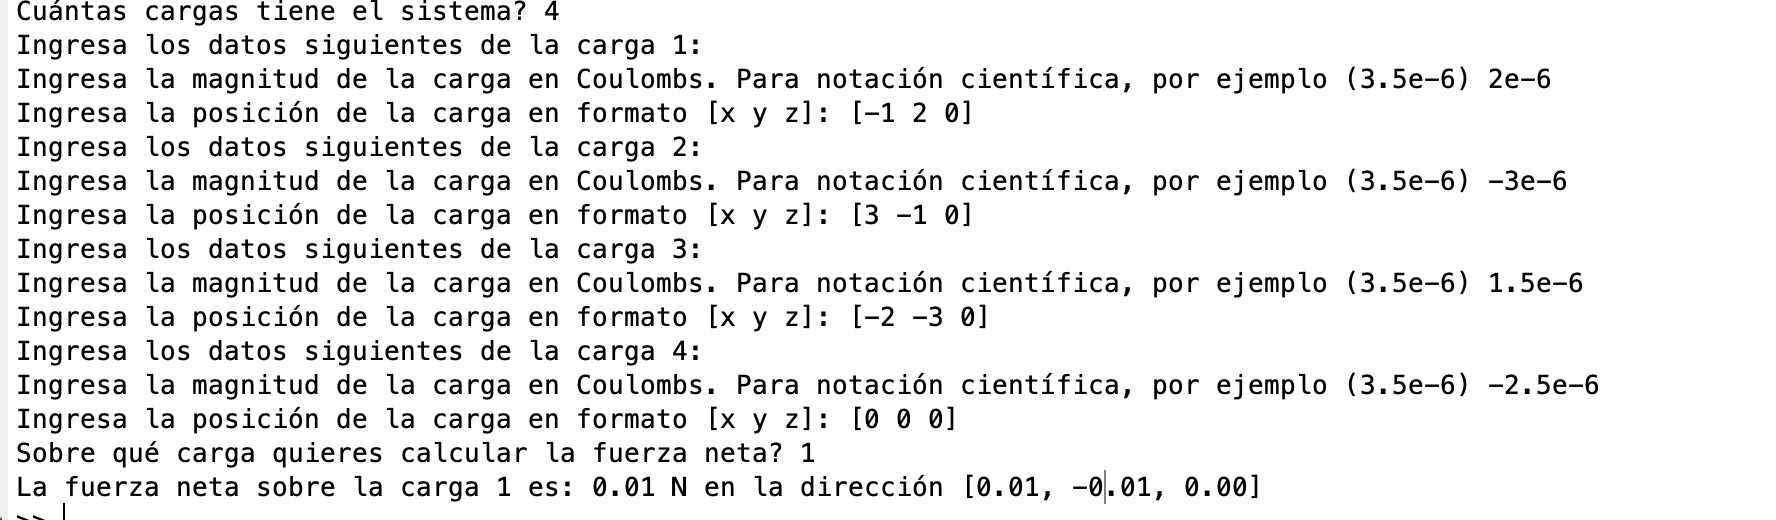
\includegraphics[height = 4cm]{2024-04-11_Prueba2SimuladorCoulomb.png}
    \caption{Cuatro cargas en el plano $xy$, tanto negativas como positivas}
    \label{fig:fig_2}
\end{figure}
En la figura \ref{fig:fig_2}, el usuario ingresa 4 cargas con sus posiciones en el plano $xy$. Los resutlados nos dicen que la fuerza resultante sobre 
la carga 1 es de $0.01N$ en la dirección $[0.01, -0.01, 0.00]$. Esto es coherente ya que la fuerza es repulsiva debido a que es positiva, además de que 
tiene componente en $x$ y $y$. 

\item Caso de prueba con $Q_1 = 3x10^{-6}C$, $Q_2 = -4x10^{-6}C$, $Q_3 = 2.5x10^{-6}C$, $Q_4 = -1.8x10^{-6}C$. Además, las magnitudes son $Q_1 = (2, 3, 1)$, $Q_2 = (-1, -1, 2)$, 
$Q_3 = (0, 5, -1)$, $Q_4 = (-3, 0, 3)$. A continuación la ejecución del programa: 
\begin{figure}[H]
    \centering
    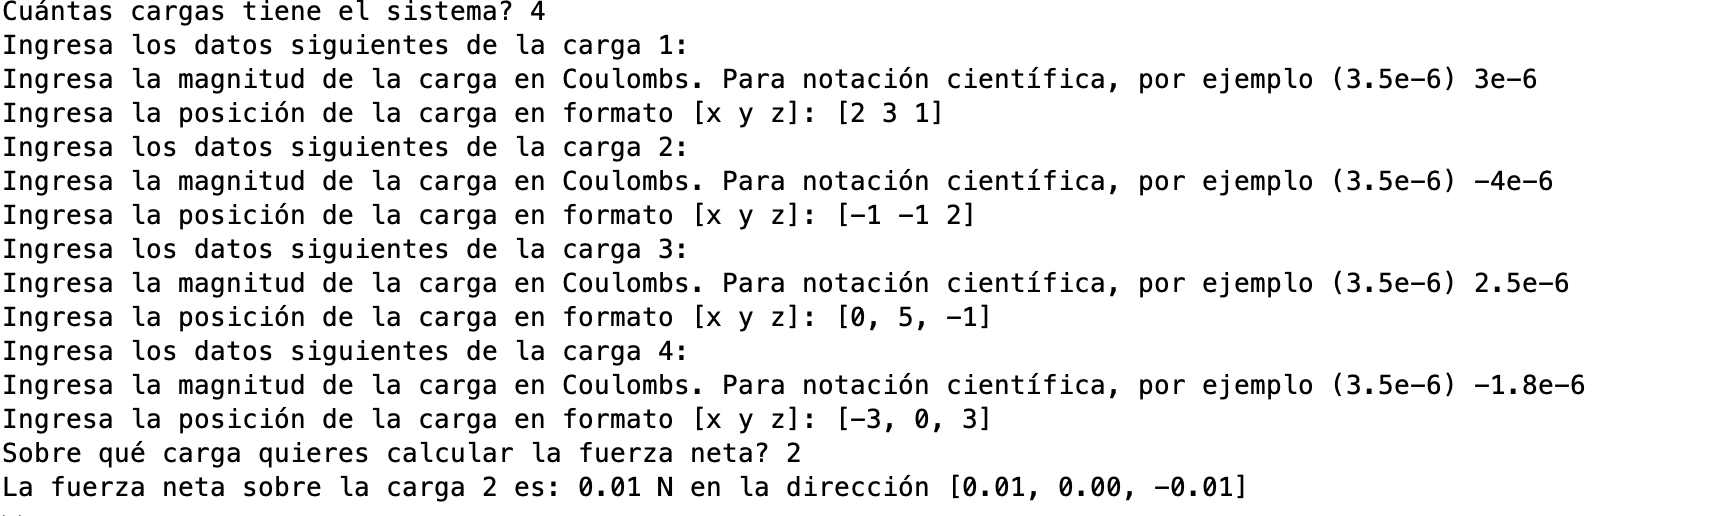
\includegraphics[height = 4cm]{2024-04-11_Prueba3SimuladorCoulomb.png}
    \caption{Cuatro cargas en el plano $xyz$, tanto negativas como positivas}
\end{figure}
Aquí, nos muestra que, la fuerza neta en la carga 2 tiene magnitud $0.01N$, y tiene componente en $x$ y en $z$, pero no en $y$. Lo cuál es consistente ya que 
nos muestra que es posible que haya fuerzas que se anulen en el eje $y$.
\end{enumerate}
\end{document}